% Beamer Presentation and Lecture Note Template
% Version 0.1
% by Paul Vesey

\mode<presentation> {
\usetheme{Antibes}
\setbeamercovered{invisible}
\setbeamertemplate{footline}[frame number]
\setbeamertemplate{navigation symbols}{} 
}

\usepackage{eurosym}
\usepackage{graphicx}
\usepackage{wasysym}
\usepackage{hyperref}
\usepackage{amsmath}
\usepackage{amssymb}
\usepackage{mathtools}
\usepackage{tikz}
\usepackage{pgf}
\usepackage{pgfplots}
\usepackage{pxfonts}
\usepackage{textcomp}
\usepackage{verbatim}
\usepackage{color}
\usepackage{xcolor}
\usepackage{fix-cm}


\author{Paul Vesey}
\institute[LIT]
{
Limerick Institute of Technology \\
\medskip
{\emph{paul.vesey@lit.ie}}
}
\date{Spring 2021}

%
\title[Project Management]{Project Integration Management}
%


\begin{document}
%

\tableofcontents
\newpage



\begin{frame}
\titlepage
\end{frame}\begin{center}\line(1,0){250}\end{center}
%
%








\section{Project Integration Management}

\subsection{Introduction}








\begin{frame}
\frametitle{Project Integration Management}
Project Integration Management Spans the 5 PM Process Groups of:
\begin{enumerate}
	\item Initiating
	\item Planning
	\item Executing
	\item Monitoring \& Controlling
	\item Closing
\end{enumerate}
\textit{It is the first of the 10 PM Knowledge Areas that we will cover.}
\end{frame}\begin{center}\line(1,0){250}\end{center}
%
%


\begin{frame}
\frametitle{Develop Project Charter}
The Project Charter is the document that formally authorises the project.\\
The Project Manager should be appointed at this stage\\
Projects are usually chartered and authorised external to the project organisation by an enterprise, government agency, a program organisation, or a portfolio organisation due to:
\begin{itemize}
	\item Market Demand (e.g. Housing Projects)
	\item Business Need (e.g. New Offices, New IT system)
	\item Customer Request (e.g. Construction Contracting)
	\item Technological Advance (e.g. Broadband Cabling)
	\item Legal Requirement (e.g. change in air emissions regulations.)
	\item Social Need (e.g. Water Treatment Plant)
\end{itemize}
\end{frame}\begin{center}\line(1,0){250}\end{center}
%
%
\begin{frame}
\frametitle{Develop Project Charter}
Developing a charter links the project with the overall goals and strategy of the company (if you can't link it, why do it?)\\
Project Charter is primarily concerned with:
\begin{itemize}
	\item Documenting business need
	\item Project justification
	\item Current understanding of customers requirements
	\item Product, service, or result to satisfy the above
\end{itemize}
\end{frame}\begin{center}\line(1,0){250}\end{center}
%
%

\begin{frame}
\frametitle{Develop Project Charter}
The project charter should address the following:
\begin{itemize}
	\item Requirements that satisfy customer, sponsor, and other stakeholders needs, wants and expectations
	\item Business Needs, high level project description
	\item Project purpose or justification
	\item Assigned Project Manager and authority level
	\item Summary milestone schedule
	\item Stakeholder influences
	\item Functional organisation \& their participation
	\item Organisational, Environmental and External assumptions and constraints
	\item Business Case justifying project; ROI etc
	\item Summary Budget
\end{itemize}
\end{frame}\begin{center}\line(1,0){250}\end{center}
%
%


\begin{frame}
\frametitle{Develop Project Charter} 
Inputs: Refer to Book for details of:
\begin{itemize}
	\item Contract
	\item Project Statement of Work
	\item Enterprise Environmental Factors
	\item Organizational Process Assets
\end{itemize}
\begin{figure}
	\centering
 		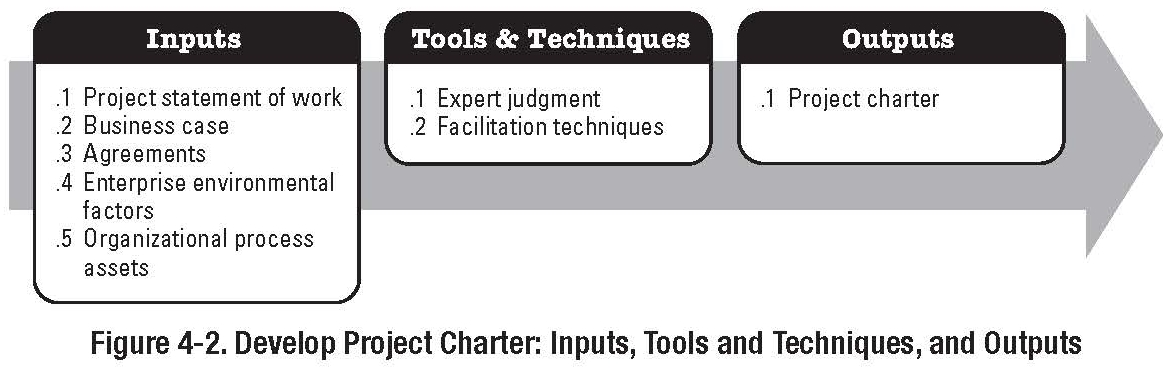
\includegraphics[width = 10cm]{images/Fig4-2.jpg}
 	\label{fig:4-2}
 \end{figure}
\end{frame}\begin{center}\line(1,0){250}\end{center}
%
%

%
%

\begin{frame}
\frametitle{Other Tools for Project Charter} 
Tools:
\begin{itemize}
	\item Project Selection Methods: Allows reader to understand why a particular project was selected
	\item Project Management Methodology: How will be project be managed and controlled
	\item Project Management Information Systems: How will information be distributed and controlled
\end{itemize}
\end{frame}\begin{center}\line(1,0){250}\end{center}
%
%

\begin{frame}
\frametitle{Project Selection Methods}
Most companies cannot execute all project proposals; selection methods help to select one project over another in a logical, rational and unbiased manner.\\
They can be:
\begin{enumerate}
	\item Mathematical models    
	\item Benefit measurement methods
\begin{itemize}
	\item Scoring Models
	\item Cash Flow Analysis Techniques    
		\begin{itemize}
			\item Payback Period
			\item Discounted Cash Flow
			\item NPV
			\item IRR
		\end{itemize}
	\item Cost-Benefit Analysis    
\end{itemize}
\end{enumerate}
	
\end{frame}\begin{center}\line(1,0){250}\end{center}
%

%

\begin{frame}
\frametitle{PM Methodology \& PM Information System}
May look similar, but very different\\
\textbf{Methodologies} are PMBOK or similar: May be formal (PMBOK) or an informal technique\\
\textbf{Information Systems} are generally software tools and techniques that provide details of resources \& activities; allow the distribution of information; and assist in scheduling and tracking.  Methodologies utilize information systems.
\end{frame}\begin{center}\line(1,0){250}\end{center}
%
%


\subsection{Develop Project Management Plan}

%
\begin{frame}
\frametitle{Develop Project Management Plan}
\begin{figure}
	\centering
		\includegraphics[width = 10cm]{images/fig4-3.jpg}
	\label{fig:4-3}
\end{figure}
\end{frame}\begin{center}\line(1,0){250}\end{center}




\begin{frame}
\frametitle{Develop Project Management Plan}
Output is the Project Management Plan
\begin{itemize}
	\item The PM Plan is a top level document that details how the project will be managed.
	\item The PM plan is managed throughout the Project
\end{itemize}
It is a `live' document.  (Version Control is vital)\\
Changes to the PM plan are made through the Integrated Change Control Process\\
The level of information contained within the plan will vary with the complexity of the project\\
The Project Plan is likely to contain processes and procedures that are common to a company's project portfolio or project programme\\
\end{frame}\begin{center}\line(1,0){250}\end{center}
%
%


%
%

\begin{frame}
\frametitle{Project Management Plan}
The Project Management Plan defines how the project is executed, monitored \& controlled, and closed.  
\begin{itemize}
	\item PM plan can be summary level or detailed and can be comprised of one or more subsidiary plans and/or other components.
	\item For construction projects, the PM Plan usually does comprise of subsidiary plans
\end{itemize}	
	
\end{frame}\begin{center}\line(1,0){250}\end{center}
%
%


\begin{frame}
\frametitle{Project Management Plan}
\begin{itemize}
	\item Defines the processes that will be used for the project
		\begin{itemize}
			\item States the degrees of execution of each process; the tools \& techniques from each process; Essential Inputs \& Outputs
		\end{itemize}
	\item Documents the dependencies and interactions of the PM processes used to manage the project
	\item Methods for executing the work to fulfill objectives
	\item Methods of monitoring and controlling change
	\item Methods to perform configuration management
	\item Methods for determining and maintaining the validity of performance baselines
	\item Communication needs of the stakeholders
	\item Project Life Cycle, Phases for multi-phase projects
	\item Management reviews of issues and pending decisions
\end{itemize}
\end{frame}\begin{center}\line(1,0){250}\end{center}
%
%


\begin{frame}
\frametitle{Project Management Plan \hfill Subsidiary Plans}
Typically:	
\begin{itemize}
	\item Project Scope Management Plan
	\item Schedule Management Plan
	\item Cost Management Plan
	\item Quality Management Plan
	\item Process Improvement Plan
	\item Staffing Management Plan
	\item Communication Management Plan
	\item Risk Management Plan
	\item Procurement Management Plan
\end{itemize}
\end{frame}\begin{center}\line(1,0){250}\end{center}
%
%
\begin{frame}
\frametitle{Project Management Plan \hfill Other Elements}
\begin{itemize}
	\item Milestone List
		\begin{itemize}
			\item Vital on construction projects
		\end{itemize}
	\item Resource Calendar
		\begin{itemize}
			\item Identifies working/non-working days in general and for individual resources
		\end{itemize}
	\item Schedule Baseline
	\item Cost Baseline
	\item Quality Baseline
	\item Risk Register
\end{itemize}
\end{frame}\begin{center}\line(1,0){250}\end{center}
%
%

\begin{frame}
\frametitle{Project Management Plan \hfill Dependencies}
The top level Project Management Plan contains elements of each of the individual subsidiary plans.\\
One of the key elements of the top-level plan is that it `maps out' the dependencies between the various processes.\\
\begin{itemize}
	\item i.e. if you identify a schedule overrun (Schedule Management) you can quickly ascertain the impacts in other plans and processes such as the cost management plan, procurement management plan etc.
	\item Any and all changes must be run through the change control process.
\end{itemize}
\end{frame}\begin{center}\line(1,0){250}\end{center}
%
%
\begin{frame}
\frametitle{Develop PMP \hfill Tools and Techniques}
Expert Judgment:
\begin{itemize}
	\item Tailor the process to meet project needs
	\item Develop technical and management details to be included in the plan
	\item Determine resources and skill levels needed
	\item Define the level of configuration management to apply
	\item Determine which project documents will be subject to change control processes
		\begin{itemize}
			\item Drawings, specs, minutes of meetings
		\end{itemize}
\end{itemize}
\end{frame}\begin{center}\line(1,0){250}\end{center}
%
%



\begin{frame}
\frametitle{Configuration Management System and Change Control System}
Both are subsets of the overall PM information system.\\
Configuration Management System consists of processes:\\ 
\begin{itemize}
	\item for  submitting proposed changes
	\item that include a tracking system for reviewing and approving or rejecting changes
	\item that define approval levels for authorising changes
	\item that define a method of validating approved changes
\end{itemize}
Normally the Configuration Management System includes the change control system - however sometimes (rarely) it is separated
\end{frame}\begin{center}\line(1,0){250}\end{center}
%
%



\begin{frame}
\frametitle{Configuration Management System}
The Configuration Mgt System is a collection of formal procedures used to apply technical and administrative direction and surveillance to:
\begin{itemize}
	\item Identify and document the functional and physical characteristics of a product or component 
		\begin{itemize}
			\item Design Drawings, Specs, etc.
		\end{itemize}
	\item Control any changes to these characteristics
		\begin{itemize}
			\item Changes to design (move a door) or changes to spec (change the door handles being used)
		\end{itemize}
	\item Record and Report each change and its implications
		\begin{itemize}
			\item Necessary for final accounts (read the contract)
			\item May have cost, safety or schedule implications
		\end{itemize}
	\item Support the audit of the products or components to verify conformance to requirements
\end{itemize}
\end{frame}\begin{center}\line(1,0){250}\end{center}
%
%

\begin{frame}
\frametitle{Change Control System}
Change Control System is a collection of documented procedures that define how project deliverables and documentation are:
\begin{itemize}
	\item Controlled, Changed, and Approved.
\end{itemize}
Control 
\begin{itemize}
	\item Who has the documents and ensuring the correct version is where it should be.
	\item Normally controlled documents have a formal list of recipients - `Controlled Copies' are normally marked as such. 
	\item May define a requirement that all controlled copies of superseded drawings and specs are returned to the main contractor or employer for destruction;  
\end{itemize}
\end{frame}\begin{center}\line(1,0){250}\end{center}
There is no point in having the latest version of a detail drawing sitting in a filing cabinet at the head office of a large construction firm; it needs to be on site also. If you are looking at version A of a document how do you know there is not a version B?
%





\begin{frame}
\frametitle{Documentation Control}
Documentation Issue and Approval
\begin{figure}
	\centering
		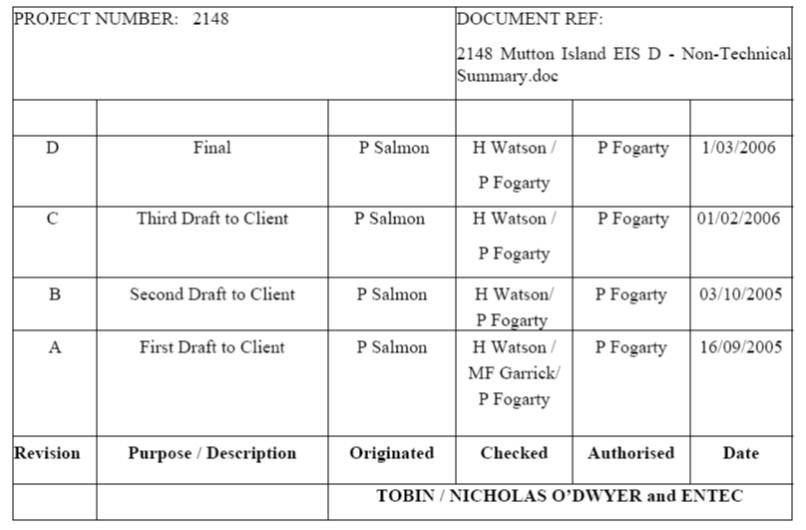
\includegraphics[width = 7cm]{images/doccontrol.jpg}
	\label{fig:doccontrol}
\end{figure}Extracted from Environmental Impact Statement,  Mutton Island Upgrade Project 
\end{frame}\begin{center}\line(1,0){250}\end{center}
%
%
%

\subsection{Monitor and Control Project Work}


\begin{frame}
\frametitle{Monitor and Control Project Work}
\begin{figure}
	\centering
		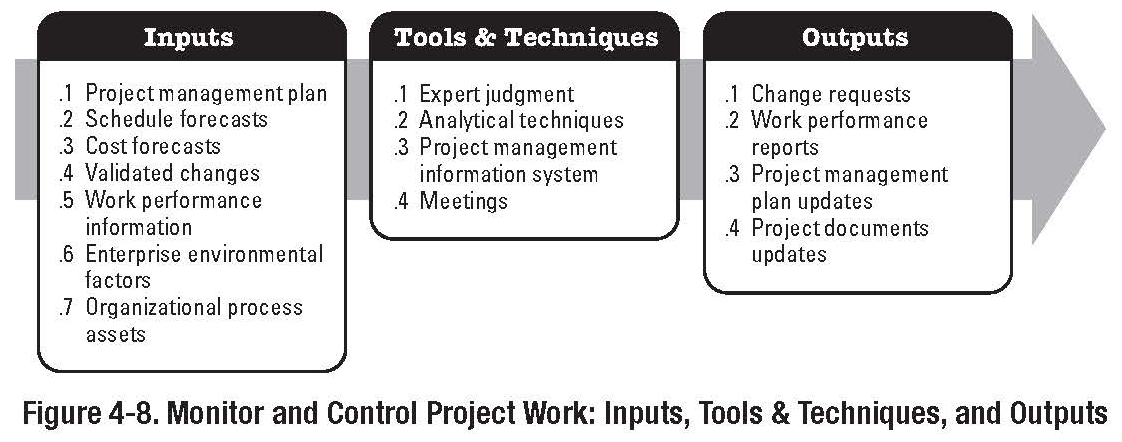
\includegraphics[width = 10cm]{images/Fig4-8.jpg}
	\label{fig:4-8}
\end{figure}Part of the Monitoring and Controlling Process Group
\end{frame}\begin{center}\line(1,0){250}\end{center}
%
%

\begin{frame}
\frametitle{Monitor and Control Project Work}
Involves:
\begin{itemize}
	\item Comparing Actual Performance against Planned Project Performance and PM Plan
	\item Assessing Performance to determine if corrective or preventative actions are required
	\item Analysing, Tracking and Monitoring Project Risks; and documenting findings
	\item Maintaining Accurate Information and ensuring that it can be retrieved in a timely manner
	\item Providing Information for Status Reporting
	\item Providing Forecasts to cost and schedule models and plans
	\item Monitoring the implementation of approved changes
\end{itemize}
\end{frame}\begin{center}\line(1,0){250}\end{center}
%
%
\begin{frame}
\frametitle{Monitor and Control Project Work}
Inputs:
\begin{itemize}
	\item Project Management Plan
	\item Performance Reports
	\item Enterprise Environmental Factors
	\item Organisational Process Assets
	\begin{itemize}
		\item Financial Systems (Purchasing, et al)
	\end{itemize}
\end{itemize}
\end{frame}\begin{center}\line(1,0){250}\end{center}
%
%

\begin{frame}
\frametitle{Monitor and Control Project Work}
Tools and Techniques:
\begin{itemize}
	\item Expert Judgement
	\item Project Management Methodology
		\begin{itemize}
			\item Methodology used by the PM team to ensure that the project is being executed in accordance with the PM Plan
		\end{itemize}
	\item Project Management Information System
		\begin{itemize}
			\item Also used for forecasts
		\end{itemize}
	\item Earned Value Management System
		\begin{itemize}
			\item Used to determine current project status, past performance and likely future performance 
		\end{itemize}
\end{itemize}
 
\end{frame}\begin{center}\line(1,0){250}\end{center}
%
%

\begin{frame}
\frametitle{Monitor and Control Project Work}
Outputs:
\begin{itemize}
	\item Change Requests
		\begin{itemize}
			\item Corrective Actions - Documented recommendations required to bring expected future project performance into conformance
			\item Preventative Actions - Documented recommendations that reduce the probability of non-conformance events
			\item Recommended Defect Repair - Repair of Defects or non-conformances identified during Quality Management
		\end{itemize}
	\item Project Document Updates - Forecasts
		\begin{itemize}
			\item ECT, EAC, Projected Completion Date etc.
		\end{itemize}
	\item Project Management Plan Updates
\end{itemize}
\end{frame}\begin{center}\line(1,0){250}\end{center}
%
%



\subsection{Perform Integrated Change Control}



\begin{frame}
\frametitle{Perform Integrated Change Control}
\begin{figure}
	\centering
		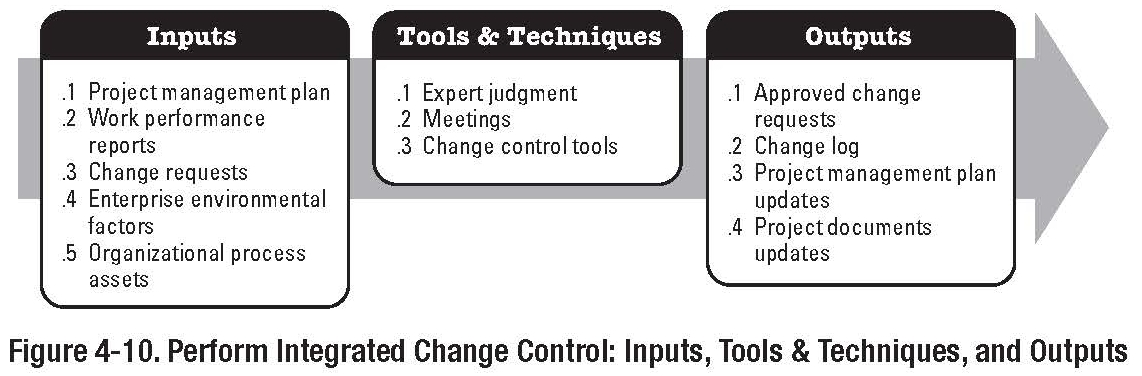
\includegraphics[width = 10cm]{images/Fig4-10.jpg}
	\label{fig:4-10}
\end{figure}Part of the Monitoring and Controlling Process Group
\end{frame}\begin{center}\line(1,0){250}\end{center}
%
%

\begin{frame}
\frametitle{Perform Integrated Change Control}
Integrated Change Control is required throughout the project lifecycle\\
PM Plan, Scope Statement, Specifications need to be controlled and maintained throughout the course of the project.
\begin{itemize}
	\item \textbf{Progressive Elaboration}
\end{itemize}
Changes requests can be either \textbf{rejected} or \textbf{approved}
\end{frame}\begin{center}\line(1,0){250}\end{center}
It is important to deal with all requests.  Generally putting items off until a later date is not advised, as it tends to lead to backlogs of work.

%
%

\begin{frame}
\frametitle{Perform Integrated Change Control}
Change Management Activities:
\begin{itemize}
	\item Identifying that a change needs to occur or has occurred
	\item Influencing the factors that circumvent integrated change control so that only approved changes are implemented
\begin{itemize}
	\item Scope Creep
\end{itemize}
	\item Reviewing and approving requested changes
	\item Managing the approved Changes when and as they occur
	\item Maintaining the integrity of baselines by releasing only approved changes
\begin{itemize}
	\item Approved changes typically modify baseline information
\end{itemize}
	\item Reviewing and Approving all recommended corrective and preventative actions
\end{itemize}
 
\end{frame}\begin{center}\line(1,0){250}\end{center}
%
%

\begin{frame}
\frametitle{Perform Integrated Change Control}
Change Management Activities:
\begin{itemize}
	\item Coordinating change across the entire project
		\begin{itemize}
			\item Controlling and Updating Scope, Cost, Budget, etc., based upon approved changes
		\end{itemize}
	\item One change can effect a multitude of documents
	\item Documenting the complete impact of requested changes
		\begin{itemize}
			\item It is not always possible to predict ahead of time what the exact impact of a change may be.  An initial estimate of 2 weeks delay may prove to be inaccurate.
		\end{itemize}
\end{itemize}
\end{frame}\begin{center}\line(1,0){250}\end{center}
%
%

\begin{frame}
\frametitle{Perform Integrated Change Control}
Proposed Changes can require new or revised:
\begin{itemize}
	\item Cost estimates 
	\item Schedule activity
	\item Schedule dates
	\item Resource requirements
	\item Risk analysis and response
\end{itemize}
Also may require modification to: 
\begin{itemize}
	\item Scope
	\item Deliverables
	\item Etc.
\end{itemize}
\end{frame}\begin{center}\line(1,0){250}\end{center}
%
%

\begin{frame}
\frametitle{Perform Integrated Change Control}
Every documented requested change must be either accepted or rejected.:
\begin{itemize}
	\item Requires persons in authority
	\item Change Review Boards may be formed
\end{itemize}
\end{frame}\begin{center}\line(1,0){250}\end{center}
%
%

\begin{frame}
\frametitle{Perform Integrated Change Control}
Inputs:
\begin{itemize}
	\item Project Management Plan
	\item Work Performance Information
	\item Change Requests
	\item Enterprise Environmental Factors
	\item Organisational Process Assets
		\begin{itemize}
			\item Procedures for change control, etc.
		\end{itemize}
\end{itemize}
\end{frame}\begin{center}\line(1,0){250}\end{center}
%
%

\begin{frame}
\frametitle{Perform Integrated Change Control}
Tools and Techniques:
\begin{itemize}
	\item Expert Judgement
		\begin{itemize}
			\item Approval Authorities are assumed to posses expert judgement\ldots.
		\end{itemize}
	\item Change Control Meetings
	\item Both Will normally require Information Systems
\end{itemize}
\end{frame}\begin{center}\line(1,0){250}\end{center}
%
%

\begin{frame}
\frametitle{Perform Integrated Change Control}
Outputs:
\begin{itemize}
	\item Change Request Status Updates
		\begin{itemize}
			\item Approved Change Requests
			\item Rejected Change Requests
			\item Approved Corrective Actions
			\item Approved Preventative Actions
			\item Approved Defect Repair
		\end{itemize}
	\item Project Management Plan Updates
	\item Project Document Updates
\end{itemize}
\end{frame}\begin{center}\line(1,0){250}\end{center}
%
%



\subsection{Close Project or Phase}



\begin{frame}
\frametitle{Close Project or Phase}
\begin{figure}
	\centering
		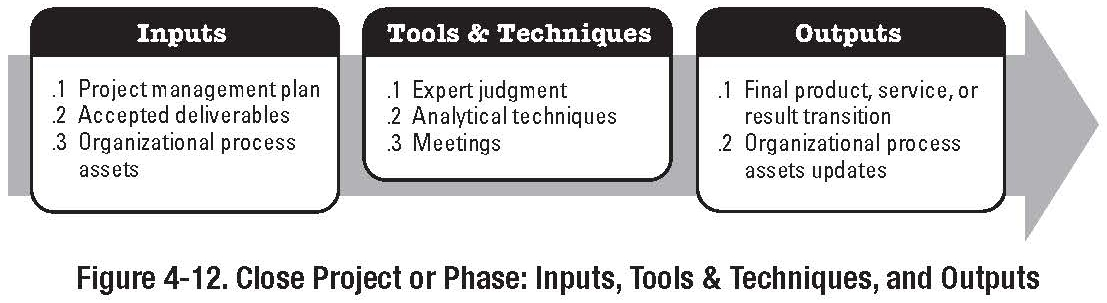
\includegraphics[width = 10cm]{images/Fig4-12.jpg}
	\label{fig:4-12}
\end{figure}
Part of the Closing Process Group
\end{frame}\begin{center}\line(1,0){250}\end{center}
%
%

\begin{frame}
\frametitle{Close Project}
Close Project involves performing the project closure portion of the PM Plan.\\
The `Close Project' process can be applied to the project as a whole but may also be applied to a project phase\\
Usually involves verifying and documenting project deliverable acceptances\\
However sometimes it involves documenting why a project was terminated before completion\\
Two main activities\\
\begin{itemize}
	\item Administrative Closure Procedure
	\item Contract Closure Procedure
\end{itemize}
\end{frame}\begin{center}\line(1,0){250}\end{center}
%
%

\begin{frame}
\frametitle{Close Project}
\textbf{Administrative Closure}
\begin{itemize}
	\item Collection of Project Records
	\item Success/Failure Analysis
	\item Lessons Learned
	\item Archiving of Project Information
\end{itemize}
\textbf{Contract Closure}
\begin{itemize}
	\item Activities required to settle or close the contract
		\begin{itemize}
			\item TOC; Completion Cert; Defects Liability Period, etc.
		\end{itemize}
	\item Requires verification of project (product) acceptance
\end{itemize}
\end{frame}\begin{center}\line(1,0){250}\end{center}
%




\end{document}



